
\section{Background and Related Work}


\subsection{Microscaling Data Formats} 
The concept of block data representation was introduced to collectively represent groups of values using shared scaling factors \cite{darvish2023shared}. 
Building on this idea, Rouhani \emph{et al.}~\cite{rouhani2023microscaling} proposed the Microscaling (MX) data format as a specific variant of block data formats, where each block of elements shares a common scale encoded in an \texttt{E8M0} power-of-two format. MX formats have since been standardized by the Open Compute Project~\cite{rouhani2023ocp}. Recent extensions explore multi-level scaling, where scaling factors are applied hierarchically across granularities. MicroScopiQ~\cite{Microscopiq} adopts a two-level scaling scheme with coarse block-level and finer micro-block-level scales, while NVFP4 \cite{abecassis2025pretraining} employs a similar hierarchy, using a tensor-level \texttt{E8M23} scale and block-level \texttt{E4M3} scale. To balance hardware complexity and software performance, we adopt a single-level scaling scheme in our configurable MX data format, with tunable parameters $(M, E, S, B)$ for MXFP and $(M, S, B)$ for MXINT, illustrated in \Cref{fig:MX_Dataformats}.

\begin{figure}[h]
  \centering
  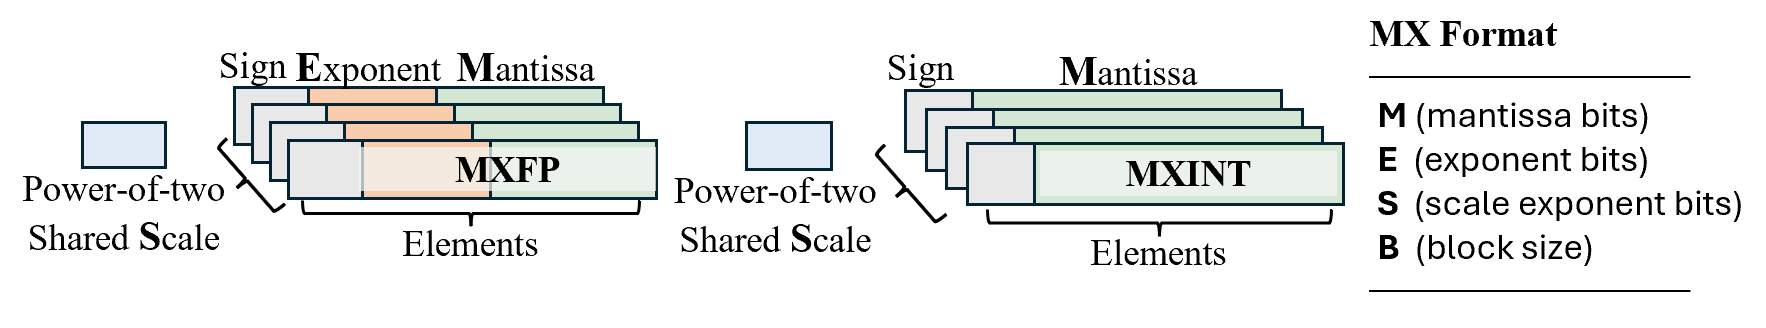
\includegraphics[width=1\linewidth]{Figures/mx_annotated.png}
  \caption{Illustration of the configurable MX data format design, parameterized with tunable configs. Each block of elements shares a power-of-two scaling factor and supports both integer and minifloat data types.}
  \label{fig:MX_Dataformats}
  \vspace{-10pt}
\end{figure}

\subsection{Co-designing PTQ with Microscaling Data Formats}

Existing off-the-shelf Post-Training Quantization (PTQ) methods are well-studied for integer data formats \cite{frantar2022gptq, QuaRot}. However, we find that these methods are less explored—and in some cases, not directly applicable—to the MX data format. 

GPTQ \cite{frantar2022gptq} was originally developed for integer quantization. We explore its adaptation to our parameterized MX data formats and propose a variant method that better adapts it to the MX format. Details are deferred to~\Cref{subsec:weights_quant}. Rotation-based PTQ methods are among the most effective techniques for mitigating activation outliers. QuaRot~\cite{QuaRot} demonstrated that the application of the Hadamard transformation can effectively suppress such outliers. However, we empirically experimented and found that without careful treatment, the direct application of these methods can lead to significant model performance degradation for MX data formats. Details are deferred to~\Cref{subsec:act_quant}.
Overall, our co-designed PTQ and data format achieves performance competitive with full-precision baselines, even under aggressive low-bit settings, as demonstrated in~\Cref{subsec:quantization_experiments}.

\begin{figure*}[t]
  \centering
  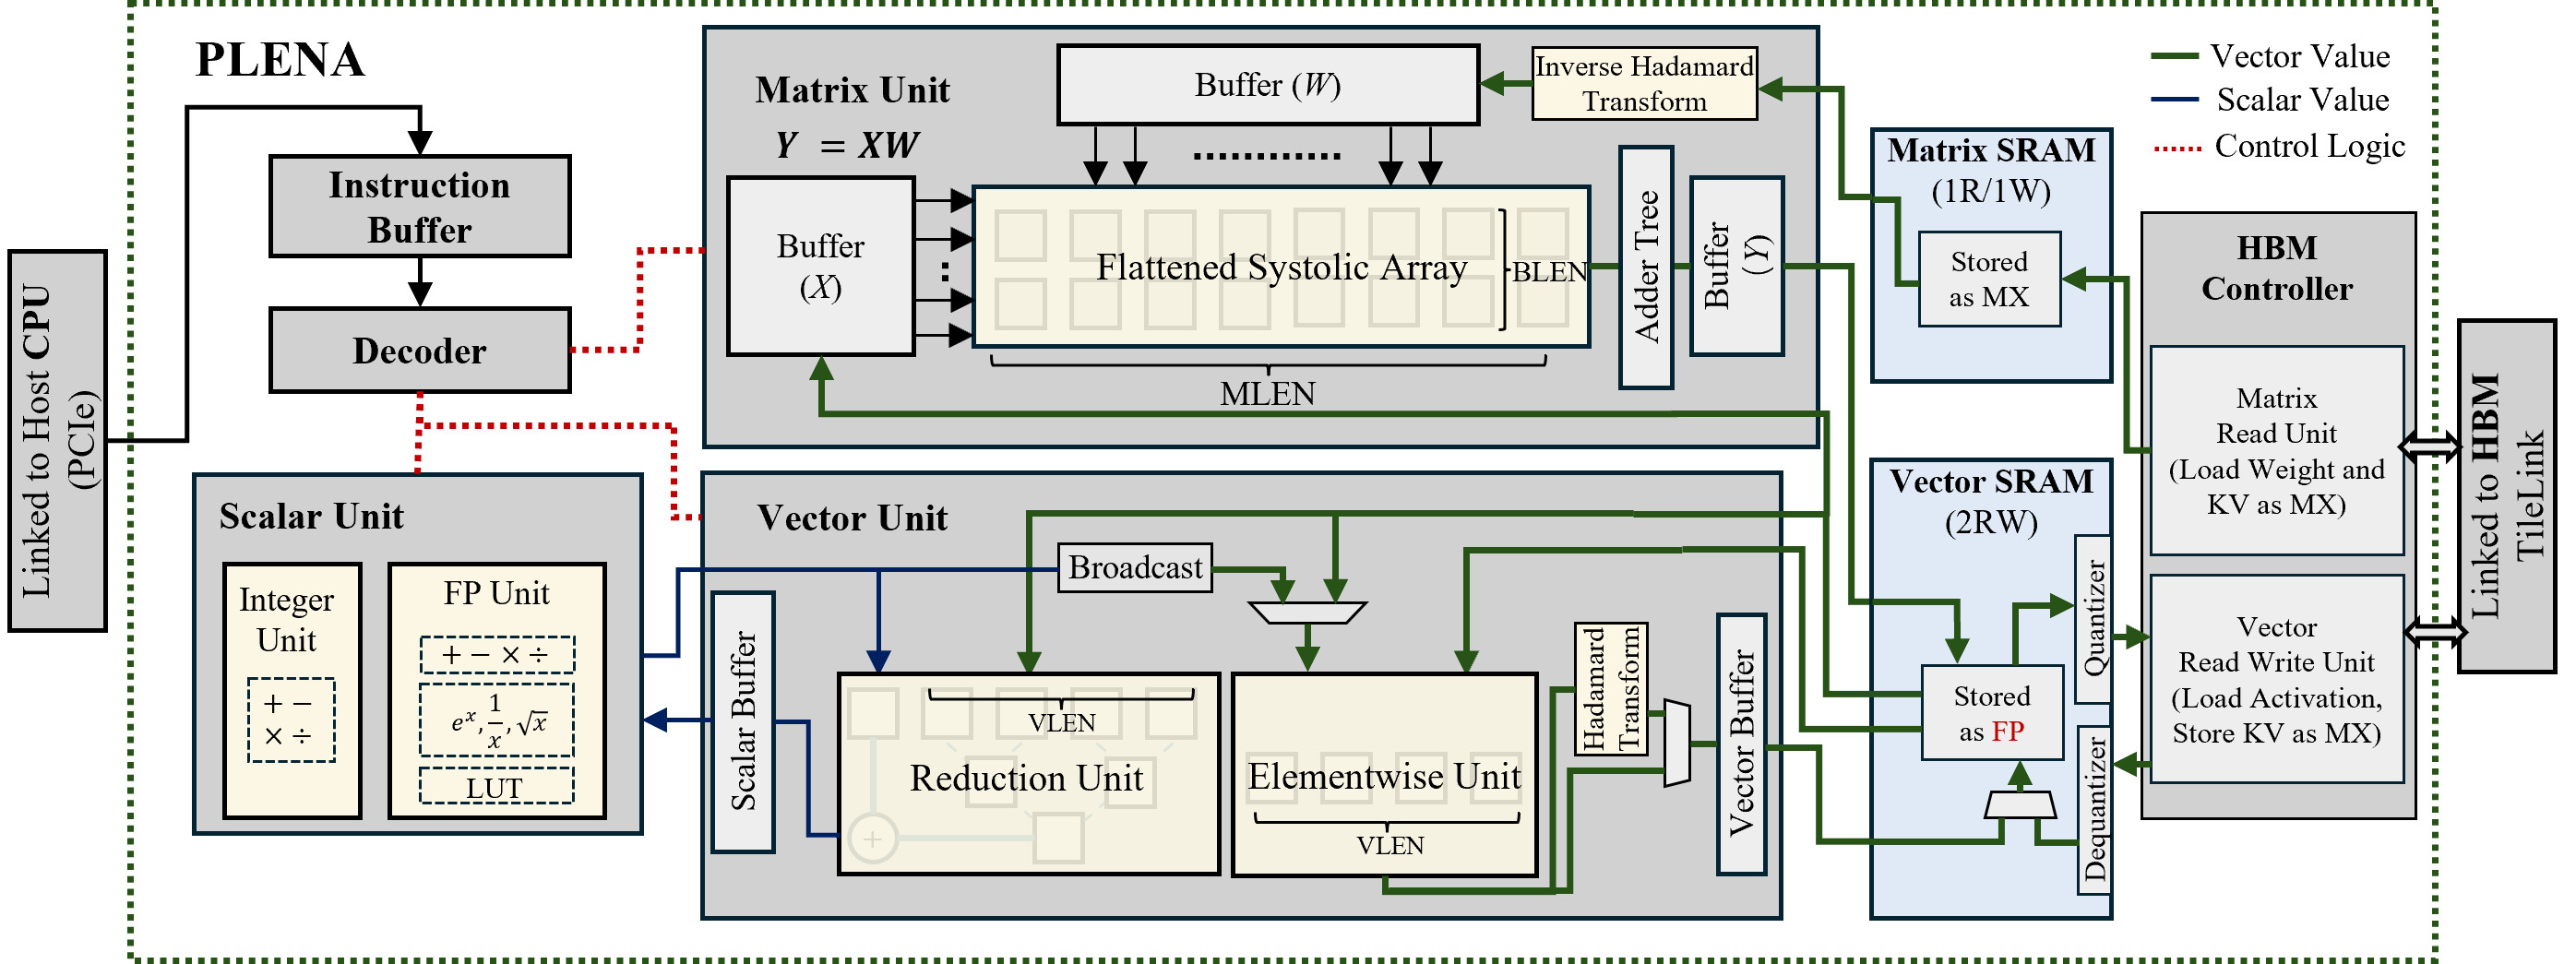
\includegraphics[width=0.96\textwidth]{Figures/Accelerator_Config.png}
  \caption{PLENA accelerator architecture overview. Execution is controlled by the decoder’s system-pipeline controller, which derives control signals from decoded instructions and monitors memory dependencies. For example, if the current instruction needs to read from a Vector SRAM row that is still being updated by the vector or matrix unit, the controller inserts a stall to ensure correctness. Vector SRAM acts as the on-chip scratchpad to the matrix and vector units.}
  \label{fig:PLENA_arch}
\end{figure*}

\subsection{FlashAttention}

FlashAttention optimizes memory I/O in the standard attention layer~\cite{FlashAttention}. In a standard attention layer, computing \(QK^{\top}\) produces a prohibitively large square matrix, often thousands by thousands in size. Because on-chip memory cannot hold this intermediate result, it must be written to off-chip memory and later reloaded for the subsequent softmax and \(PV\) steps, which significantly degrades performance. FlashAttention avoids this round trip by tiling and fusing the attention computation (GEMM–Softmax–GEMM) so that all intermediate results fit on-chip. 

Most existing systolic-array–based accelerators do not natively support FlashAttention. SystolicAttention~\cite{SystolicAttn} is among the first to integrate FlashAttention into a systolic architecture by deploying the FlashAttention into the hardware.  In contrast, PLENA adopts a more flexible approach, enabling aggressive memory prefetching overlap and leveraging a mixed-precision supported flattened systolic array with head-level decomposition to achieve higher compute utilization and efficiency. As discussed in \Cref{subsec:flashatten}, we identify three key architectural capabilities required to efficiently support FlashAttention.


\subsection{Accelerators and Their Quantization Supports}
\label{sec:accelerators}

Recent LLM accelerators~\cite{picachu, Microscopiq, FlightLLM, TENDER, FIGNA, Tandem, guo2023olive, hu2025mant, guo2022ant} explore diverse architectural trade-offs across compute organization, kernel specialization, and system integration. However, many of these designs focus on accelerating specific kernels (e.g., GEMM or attention) rather than supporting the full Transformer inference pipeline, often requiring offloading of unsupported operations to external processors. Such partial coverage can introduce additional data movement and limit sustained utilization under long-context inference workloads. PLENA instead targets full Transformer inference directly on the accelerator fabric.

Prior works have also explored hardware and quantization
co-design~\cite{zadeh2020gobo, guo2022ant, guo2023olive, Microscopiq,
hu2025mant}. MicroScopiQ~\cite{Microscopiq} adopts GPTQ for two-level
MX quantization. ANT and MANT~\cite{guo2022ant, hu2025mant} propose
hybrid data formats that adapt quantization mode to input distributions
at runtime. OliVe~\cite{guo2023olive} handles outliers by pairing them
with adjacent low-magnitude weights. However, these
works mostly focus on weight and activation quantization, without
jointly addressing KV cache quantization under long-context inference
scenarios. PLENA, by contrast, is the
first to natively support tunable MX formats with both
hardware friendly QuaRot~\cite{QuaRot} and GPTQ~\cite{frantar2022gptq} while
targeting long-context workloads natively.

Prior work such as Scale-Sim~\cite{samajdar2018scale} supports the simulation of flattened systolic arrays for DNN inference, while SARA~\cite{SARA} explores reconfigurable array shapes to optimize general DNN workloads. However, these approaches do not explicitly consider the characteristics of autoregressive Transformer inference. PLENA instead adopts a workload-driven design that reshapes the systolic organization to address the imbalance between FlashAttention and FFN computation under memory-constrained batching. The flattened array is further optimized for FlashAttention via head-level decomposition, enabling efficient acceleration of both FFN and attention during prefill and decode while maintaining high utilization for both standard and long-context (agentic) inference.

\newcommand{\myflushright}[1]{%
  \unskip\hspace*{1em plus 1fill}%
  \nolinebreak[3]\hspace*{\fill}\mbox{\upshape #1}
}

\newcommand\capped[1]{\textcolor{czblue}{\boldsymbol{#1}}}
\newcommand\varied[1]{\textcolor{czred}{\boldsymbol{#1}}}

\definecolor{nonlin}{RGB}{33,113,181}   % blue for nonlinear ops
\definecolor{linop}{RGB}{35,139,69}     % green for linear ops (RoPE)
\definecolor{matmul}{RGB}{180,15,32}    % red for matrix multiplications
\newcommand{\nonlin}[1]{\textcolor{nonlin}{\textsc{#1}}}
\newcommand{\linop}[1]{\textcolor{linop}{\textsc{#1}}}
\newcommand{\mat}[1]{\textcolor{matmul}{\textbf{[MatMul#1]}}}

